\documentclass{primus}
\usepackage{graphicx}
\usepackage{float}
\usepackage{url}

\renewcommand{\baselinestretch}{1.3}

\title{From Exam to Education: The Math Exam/Education Resources}


\keywords{education learning resource, exam database, MediaWiki, online learning, wiki}

\markboth{}{From Exam to Education: The MER}

\begin{document}
%\makePtitlepage
\makePtitle

\begin{abstract}
The Math Exam/Education Resources (MER) is an open online learning resource hosted at The University of British Columbia (UBC), aimed at providing mathematics education resources for students and instructors at UBC. In this paper, there will be a discussion of the motivation for creating this resource on the MediaWiki platform, key features of the implementation that support student learning (including the evolution of the MER wiki from an exam database to more general learning resource), data on student use and response, potential for future development, and a brief description of how the project was implemented. Preliminary correlation data between wiki usage and exam performance are shared along with some preliminary data from an ongoing impact study.
\end{abstract}

\listkeywords

\section{INTRODUCTION}\label{sec:Introduction}

The Math Exam/Education Resources (MER)\footnote{see \url{http://wiki.ubc.ca/Science:Math_Exam_Resources}} is a digital collection of material aimed at improving undergraduate students’ knowledge of mathematics with a focus on first year courses at The University of British Columbia (UBC). The project, which is maintained primarily by graduate student volunteers in the mathematics department at UBC, began as a database of examination solutions in February 2012, and since then has evolved into an extensive library of tools that students can use to study mathematics. These tools include access to detailed and peer-reviewed hints and solutions, focused topics pages that help navigate the database for specific types of problems, and also short video lectures. Furthermore, students can assign a difficulty scale to the problems they attempt and see the average rating of their peers. Embedded syllabi allow students to quickly find the relevant content for their midterm and final exams. Through thousands of students accessing the resource, a substantial amount of data has been collected on exam and course usage, as well as time periods of high traffic. This data can be used to gauge exam difficulty, to identify the amount of time and how students are spending their time studying, and to further develop the wiki to increase its effectiveness in facilitating students’ self-directed online learning.
\\\\
\noindent{}In this paper the background and implementation of the MER wiki and the particular features that contribute to its effectiveness and popularity as a learning resource are discussed. This is concluded by showing some usage statistics, including correlated data between perceived question difficulty and exam performance, and also a showcase of some preliminary results from a study into the impact of the MER on learning.  At this point it is worth emphasizing that while the project was implemented at UBC and thus the examples are taken from courses offered by that institution, the ideas and infrastructure can easily be adopted to fit any institution.  Furthermore, the concepts could even extend beyond mathematics courses to any classes where there is significant pedagogical benefit from learning with/learning via worked examples.  Therefore, the scope of this paper should be considered in terms of the information available to students, as well as the data and feedback they can provide while using such an online learning tool. 

\section{HISTORY AND RATIONALE}\label{sec:History_and_Rationale}
In the mid 1980s and early 1990s a research movement studying the usefulness of worked examples was developed to examine the effects of this technique on learning. It was shown in \cite{CS1}, \cite{CS2}, \cite{PM} that, in general, worked examples will save students time while studying and will improve test scores on both similar problems and on problems that are more advanced than the given worked example problems themselves. Thus, it can be helpful to offer students worked solutions to previous exams as a study aid. This has been the case in the mathematics department of UBC for many years.
\\\\
\noindent{}Traditionally, the mathematics department at UBC makes its exams publically available for students shortly after they are administered, albeit without solutions. Independently from the mathematics department, solutions to these exams were sold in paper copies to undergraduate students. As technology improved, the department started uploading their tests to the public department website, but the medium of solution delivery was essentially unchanged. By the static nature of the product, solution packages quickly fell out of date and were arduous to update efficiently. They were often riddled with typos and mathematical errors, and maintained a very poor quality control standard. In February 2012, a group of graduate students, dissatisfied with the aforementioned issues, concluded that most of the problems stemmed from the dissemination model and began researching alternative approaches.
\\\\
\noindent{}While dissatisfaction was growing within the graduate students regarding the exam solution delivery system, UBC was independently developing a campus-wide MediaWiki that could collectively host a variety of university initiatives and educational products. The format is probably best known for its use in Wikipedia.org, though it is a widespread online platform, used because of its intuitive structure and its ease of collaboration. Some graduate student instructors in the mathematics department had already used the UBC wiki as an effective alternative to a traditional course webpage, in particular, because of its ease in adding and editing mathematical content and formulas. Furthermore, this platform features an integrated version control which allows for the recovery of previous content if desired. These attributes were just a few of the reasons why a MediaWiki server emerged as the best option for the new dissemination model and using this technology, the MER wiki was created.
\\\\
\noindent{}One of the greatest features of the wiki is that it offers free and worldwide access, contrasting the model where hard-copy solutions were only sold on campus and only during specific times. In addition, even with the open access feature, the MediaWiki system allows us to limit editing rights to mathematics experts (primarily UBC mathematics graduate students), so that the quality of the resource can be rigorously maintained. The main tool used to maintain this quality is a peer-review flagging system, a tiered layer involving various reviews and revisions to content. Students can interact with editors and each other via discussion pages and recommend changes to the content using feedback forms. The dynamic editing process means solutions that were static and hence difficult to modify can now be easily updated to improve student understanding. This process allows the MER wiki to improve on the limitations with the aforementioned paper-based solution packages.
\\\\
\noindent{}When this project was started in February 2012, the development team focused on setting up its basic infrastructure and adding content for various first and second year undergraduate math courses at UBC\footnote{For a brief technical survey of the implementation, please see Appendix \ref{sec:Appendix}.
}. Even in this initial phase, there were immediate positive changes compared to the paper model. This new model was instantaneously wider in scope and power because the content was made more widely accessible and easier to improve. Moreover, the MER wiki featured not only solutions, but also hints and study tips, a service not available in the previous exam solution packages. These hints offered help to students wanting to complete an independent solution before looking at the answer. The impact of this small change to the product was significant. For the first time, the idea of simply offering solutions to students enrolled in undergraduate mathematics classes shifted toward an enhanced learning resource.
This notion \textemdash{} that the MER wiki was not simply providing solutions, but also resources and guidance for students learning mathematics \textemdash{} became the motivation and philosophy behind the entire project, and led to the current version of the site. The contributors began to design solutions that instructed students on how to solve problems rather than just providing the final answer, while also explaining the mathematical concepts behind the questions. A tagging system was also introduced that presents the questions grouped by topic, so students can review specific concepts and access relevant problems that might even come from different courses. To better reflect the modern philosophy of the resource, the identity of the wiki was recently changed from Math Exam Resources to the current name, Math Exam/Education Resources.
\\\\
\noindent{}At the time of writing, this project has over 1500 worked solutions spanning 17 courses and has been accessed over 1,000,000 times for a total of over 35,000 hours collectively spent on the wiki in the first two years. As the project has matured, the focus has shifted to developing the online resource as an educational product.

\section{INNOVATIVE FEATURES}\label{sec:Innovative_Features}
The MER wiki came into being as an improved alternative to a paper based dissemination model. In this section, detail is provided for key features of the implementation that make it a superior model of content dissemination and student learning.
\\\\
\noindent{}In what follows, wiki contributors are defined as those who edit wiki content, typically graduate students in the mathematics department, and users as the people who use the content in the wiki to improve their mathematical understanding, typically undergraduate students.

\subsection{DESIGN AND DESIGN INTENTION}\label{sec:Design_and_Design_Intention}
The understanding, as evidenced by student use of the wiki and usage surveys, is that students are seeking practice questions to solidify their problem-solving and computational skills. They can access questions by topic to review particular question types, or by course to simulate an exam situation. For each question, the hint(s) and solution(s) are initially hidden when the page is opened. This is designed to motivate students to solve the questions themselves before checking solutions. Each question page displays general problem solving advice (see Figure \ref{fig:question_page}), encouraging the student to try the question on their own, reveal the hint(s) if necessary, and finally reveal the solution(s) only when the problem is solved or if they are genuinely stuck.
\\\\
\noindent{}Once students have attempted a problem or have difficulties on how to approach the problem, they have the option to reveal hints to help with their problem solving strategy. Sometimes multiple hints are available, for example, when there is more than one natural way to solve a problem, or when a solution warrants many steps. A user can reveal the solution at the bottom of the page and check over their work, ideally after attempting the problem for themselves.
\\\\
\noindent{}At the end of each question, students have a chance to rate the question’s difficulty and/or provide feedback (see sections \ref{sec:Rating_Bar} and \ref{sec:Student_Feedback}). In Figure \ref{fig:question_page_annotate}, one can see a sample of this process.
\begin{figure}[H]
\centering
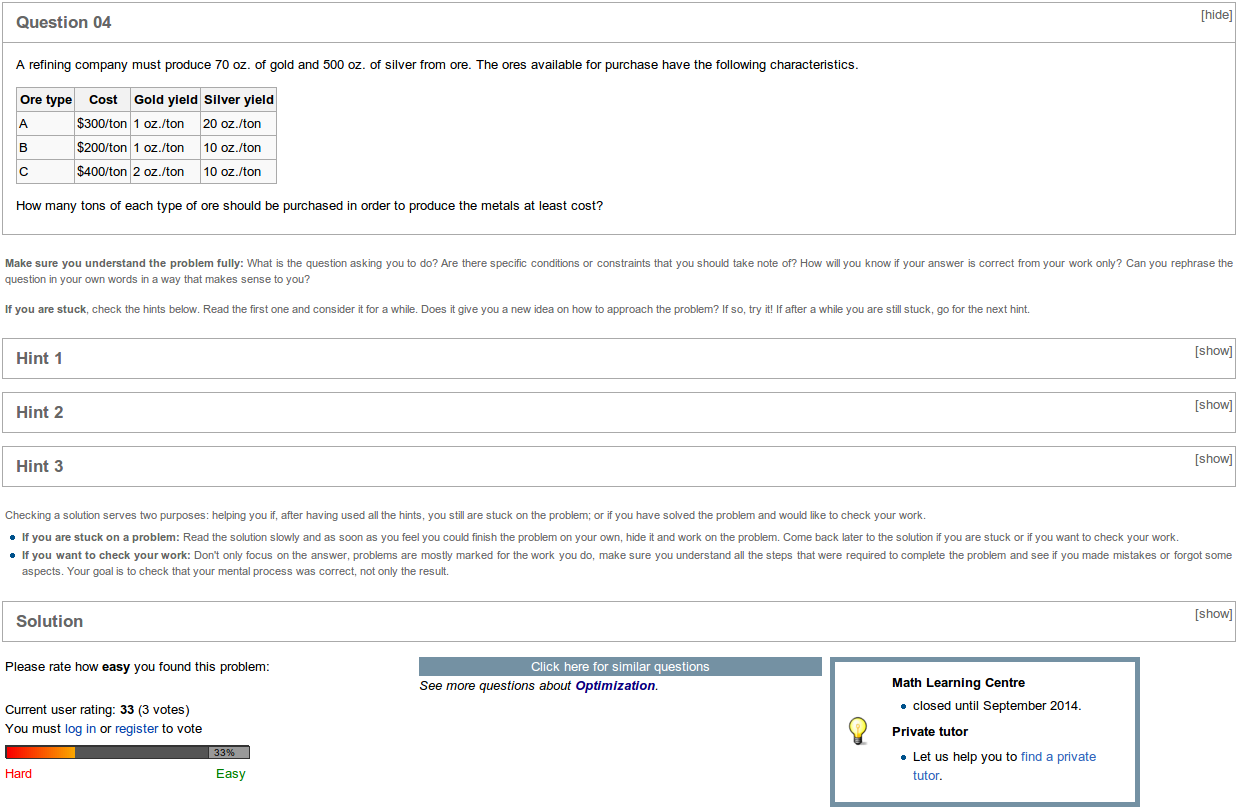
\includegraphics[width=\textwidth]{figs/Question_Page.png}
\caption{A representative example of what a student sees when they click on one of the questions in the MER wiki.}\label{fig:question_page}
\end{figure}
\begin{figure}[H]
\centering
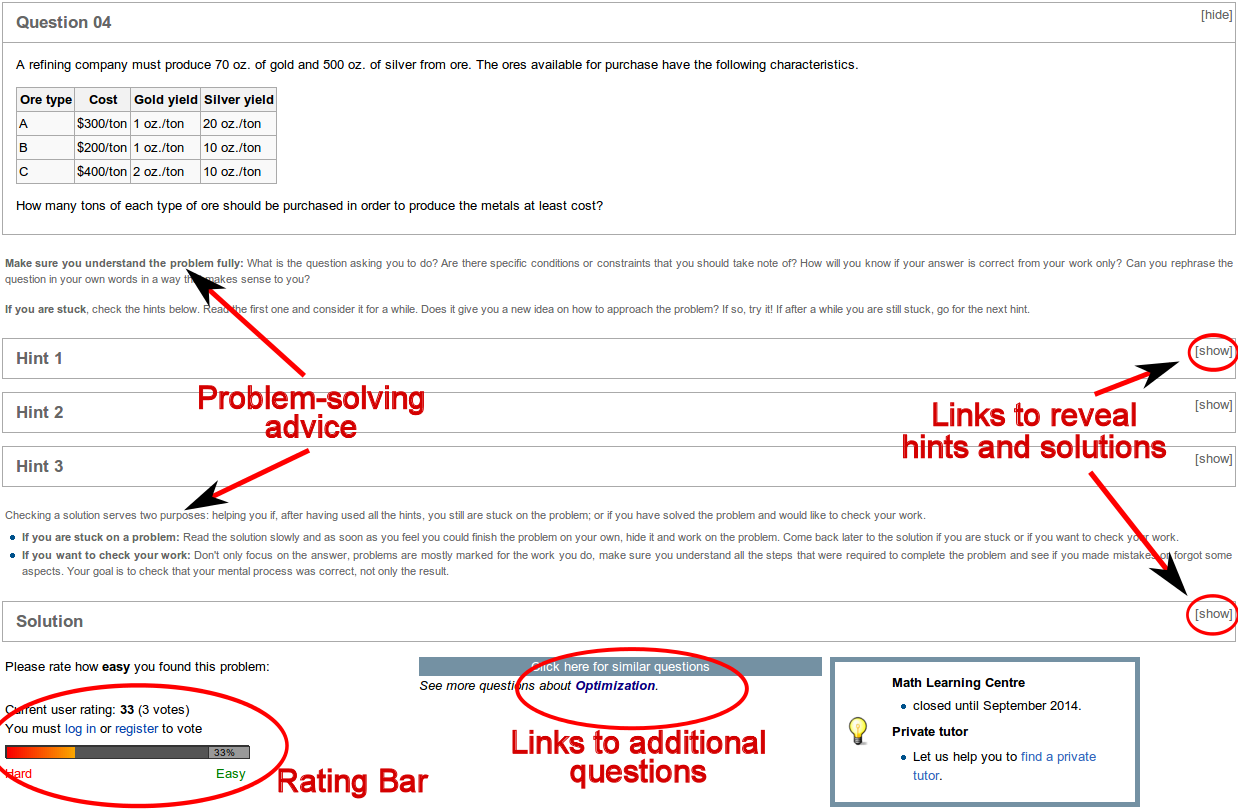
\includegraphics[width=\textwidth]{figs/Question_Page_annotated.png}
\caption{This graphic highlights several of the interactive features that students encounter on a question page.}\label{fig:question_page_annotate}
\end{figure}

\subsection{PEER REVIEW}\label{sec:Peer_Review}
One of the main advantages of the wiki system is the ability to collaboratively edit central documents. For the MER, this feature was improved by implementing a dynamic peer review process. Unlike many static methods to disseminate mathematics questions and solutions, the MER wiki content can continually be updated and improved upon; questions and solutions pass through multiple quality-filtering processes. First, there is an initial content creation phase where wiki contributors design hints and detailed solutions for an exam question. Once a wiki contributor has transcribed a question, or written a hint or solution to a problem, the content is immediately accessible to everyone, but the content is labelled with a warning that there has been no review of the contribution. Next, an open review process occurs, where the larger community of wiki contributors analyze the hints and solutions for two equally important attributes: correctness and value to the mathematical learning process. Once solutions and the corresponding hints have met the wiki’s standard of excellence, it is finally flagged as a good quality solution and indicated as such to users who visit the corresponding question page.
\\\\
\noindent{}The review process described above was motivated by the long standing use in traditional print mediums such as academic journals. On top of that, the dynamic features of the wiki multimedia platform allow for greater control in maintaining long-term quality. Quality issues can range from clarity to content correctness, as well as logical or typesetting errors. At any point in the review process, all wiki users and contributors are able to post comments on the content and suggest further improvements in the solution’s clarity or presentation, including after a solution has been deemed good quality.
\\\\
\noindent{}One such example of user-contributor interaction is shown in Figure \ref{fig:Comment_Question}. A student has studied the solution to an integration question\footnote{\label{ft:question}\url{http://wiki.ubc.ca/Science:Math_Exam_Resources/Courses/MATH103/April_2010/Question_4_(c)}} and is struggling with a concept required to solve the problem. The student posts a comment on the discussion forum and one of the contributors provides further explanation to the student using mathematical syntax. It is worth emphasizing here that the discussion page is not part of the peer review process. In this particular example, the student's question was addressed by a contributor, but comments can just as easily be made by other students to mixed quality. As such, there is not a strong focus on pedagogy for this informal framework. However, the discussions that result from a particular question often result in additions or clarifications to hints and solutions that are peer reviewed.
\\\\
\noindent{}If a solution that has been peer-reviewed and accepted is found to have an error, it can be flagged as erroneous, allowing contributors to improve the solution and re-flag it for review. This additional editing flexibility is important for many reasons. First, an incorrect solution that was erroneously accepted by a peer can later be corrected. An excellent example of this is in Figure \ref{fig:Comment_Error} where a question originally flagged as good quality has been found to have a mistake by one of the many users. A contributor was able to reply to this user, make the necessary corrections to the solution and resubmit it to the queue for review. This dynamic exchange noticeably improves on the paper exam solution packages which lacked quality control. Second, with a print model, it might not be economically viable to
correct a small calculation error. However, in an online resource where micro edits are easy, such corrections can occur quickly, cost nothing, and be available to users instantly after the update occurs.
\\\\
\noindent{}Even when a solution is correct technically, a student may comment that a solution approved as good quality is in fact difficult to comprehend, bring it to the attention of the contributors who can then improve on the clarity of the solution. This can be particularly useful if the techniques covered in class are different than those of the current solution, if the notation is unfamiliar to the students, or if a mathematical step needs further clarification. Figure \ref{fig:Comment_Suggestion} demonstrates a user asking for clarification on an alternative technique to solving a problem. A contributor then provides new insight for the student but ultimately creates an entirely new, alternative solution for the problem. Improvement could also come from a contributor's perspective where they think of an alternative hint or solution, which they can then add and flag for review.
\begin{figure}[H]
\centering
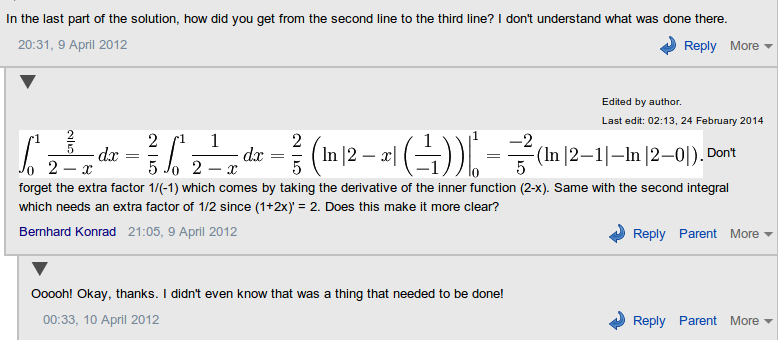
\includegraphics[width=\textwidth]{figs/Comment_Question.png}
\caption{A student uses the discussion forum to ask wiki contributors to clarify the solution presented. After a brief discussion, the matter is resolved.}\label{fig:Comment_Question}
\end{figure}
\begin{figure}[H]
\centering
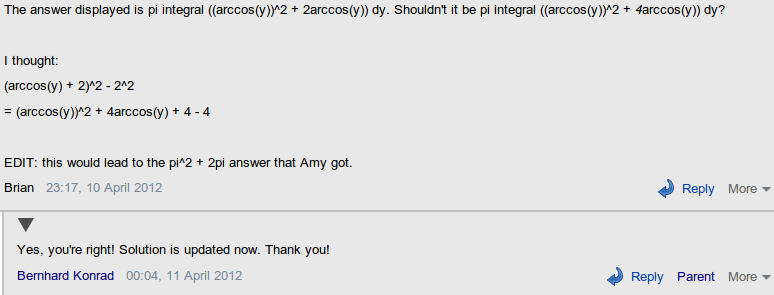
\includegraphics[width=\textwidth]{figs/Comment_Error.png}
\caption{A student finds an error in the solution and addresses it on the discussion page. Wiki contributors verify the mistake and make the appropriate corrections.}\label{fig:Comment_Error}
\end{figure}
\begin{figure}[H]
\centering
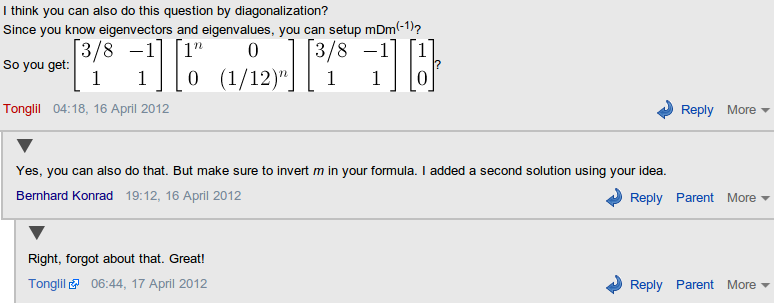
\includegraphics[width=\textwidth]{figs/Comment_Suggestion.png}
\caption{A student finds an alternative approach to solving the problem and suggests the solution on the discussion pages. A contributor acknowledges the alternative technique and creates a new secondary solution based on the student feedback.}\label{fig:Comment_Suggestion}
\end{figure}

\subsection{STUDENT FEEDBACK}\label{sec:Student_Feedback}
MediaWiki has the built-in option to comment on pages, meaning any user can comment on question pages in order to ask for help or make suggestions. However, it was noticed that the option was not being fully utilized on the wiki. This might be because commenting required a UBC-specific login that may breach the student's anonymity. To encourage more interaction, a link was embedded to a form where students can anonymously ask questions or report typos. Since this addition, significantly more errors have been pointed out and quickly fixed, and solutions were also clarified at a much higher rate. Once a student comments on a solution, a contributor can fix the error and resubmit the question to the peer review process to ensure good quality and no newly introduced typos (see Figures \ref{fig:Comment_Question}, \ref{fig:Comment_Error}, and \ref{fig:Comment_Suggestion}).

\subsection{TAGGING SYSTEM AND TOPICS PAGES}\label{sec:Tagging_System}
The tagging system on the wiki is analogous to the topic index found at the back of many textbooks. Each question is categorized based on a list of topics that are created, adapted and modified as necessary. Once a question is entered with hints and solutions, a tag is attached to the problem to identify the mathematical concept it addresses. At the time of this writing, there are over 150 different tags ranging from \textit{affine cryptosystems} to \textit{work} (Figure \ref{fig:wiki_tags}). This system is a key feature that helped propel the wiki from an exam database to an educational resource. Examination questions do not necessarily follow the same logical order that an instructor would choose to teach their course. Thus, for the wiki to be of use year-round, a tagging system was needed to help organize questions by topic. Each tag has its own wiki page where all questions of this tag are listed and organized both by course and in bulk.

\begin{figure}[H]
\centering
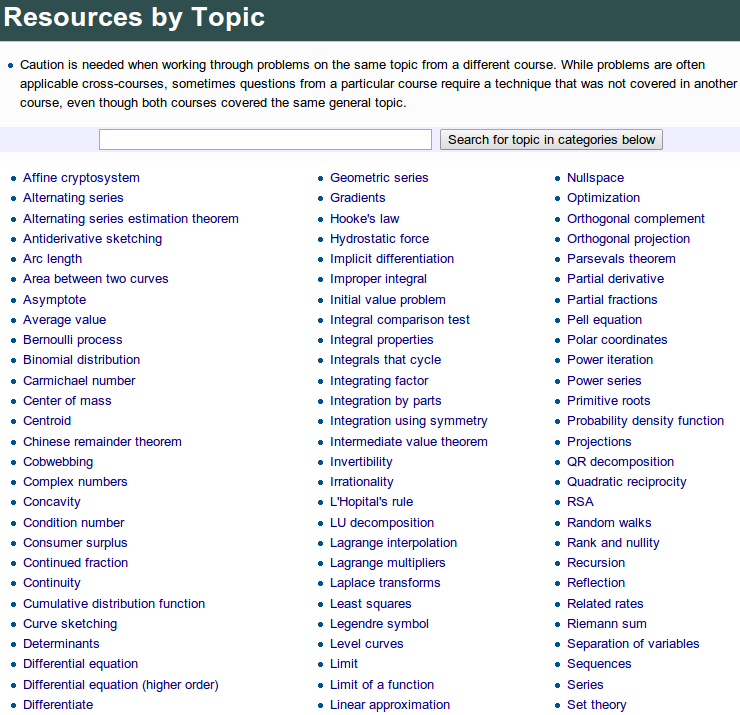
\includegraphics[width=\textwidth]{figs/Tag_List.png}
\caption{A list of topics available for study on the MER wiki up-to-date as of the writing of this paper.}\label{fig:wiki_tags}
\end{figure}

\noindent{}Being a dynamic medium, the functionality of these category page goes beyond a standard index. In particular, videos have been added on the topics pages. Videos included here range from giving concrete examples to discussing the underlying concepts in more detail, both of which help to promote student understanding. The majority of these current videos were created by Patrick Jones\footnote{see \url{http://patrickjmt.com/}} and are hosted on YouTube. Videos from local instructors are included as well and there are plans to continue to expand the database. For example, pencasts for some topic pages were recently included. The wiki can embed these videos directly on the topics pages and thus students can not only use the topic page to locate similar problems on these pages, but can also learn from videos relevant to the concept on the tagging page. A sample tag page can be found at \url{http://wiki.ubc.ca/Category:MER_Tag_Fundamental_theorem_of_calculus} (see Figure \ref{fig:topic_page}).

\begin{figure}[H]
\centering
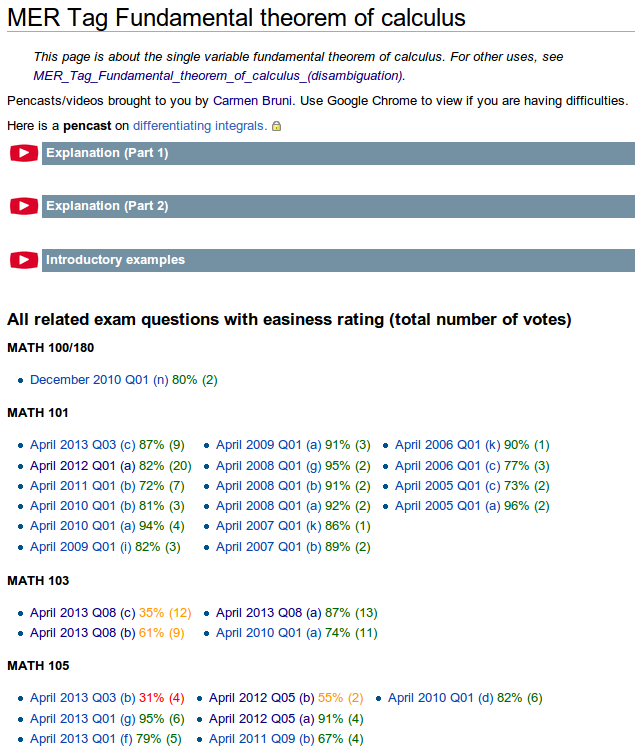
\includegraphics[width=\textwidth]{figs/Topics_Page.png}
\caption{An example of a topic page that students would access from the list in Figure \ref{fig:wiki_tags}.}\label{fig:topic_page}
\end{figure}

\noindent{}With the promotion of topics pages, the wiki saw a much heavier use during the entire term, not only around final exam period (see Section \ref{sec:Usage_Data} on the usage statistics). Students can easily obtain access to a hand-picked selection of videos and to relevant final exam problems that can help them study for midterm tests and to reinforce concepts taught in class. This is also a resource that instructors can easily direct their students toward which can be used to help get additional support in mathematics courses. For example, in a lecture of a class taught by Carmen Bruni, a student asked for another example of an ``integration-by-parts'' problem. Instead of having to design an example in class or taking one from the textbook, the instructor was able to go to the corresponding topic page on the wiki to select a relevant problem of suitable difficulty, and get his students to complete it in class. The instructor offered hints in two-minute intervals and finally revealed the step by step solution for students to verify their work. In another example, Iain Moyles was teaching a second year course that relied heavily on first year prerequisite courses currently featured on the MER wiki. When students struggled with topics from those courses, the instructor was able to direct them to various tagging pages on the wiki, eliminating the need to review prerequisite topics in class and giving the instructor the opportunity to introduce students to a free, easy-to-access, and relevant resource for their personal review.

\subsection{RATING BAR}\label{sec:Rating_Bar}
One of the more interactive aspects of the wiki is the ability for students to vote on the easiness of a question. Students can rank how easy they perceive a problem based on a 0-100 point scale (with a score of 100 indicating an extremely easy problem). In order to vote on the difficulty of a question, users must be logged into the system with their UBC account, which allows users to update their vote and prevents multiple votes from the same person (see Figure \ref{fig:Rating_bar}). Unlike the discussion page commenting previously mentioned, the rating of an individual user is not public even with logging in. At the time of writing, over 700 questions have received a total of over 3000 ratings. The average rating is displayed on every question page so that students can see how challenging their peers perceive a problem before they start their own solution attempt.

\begin{figure}[H]
\centering
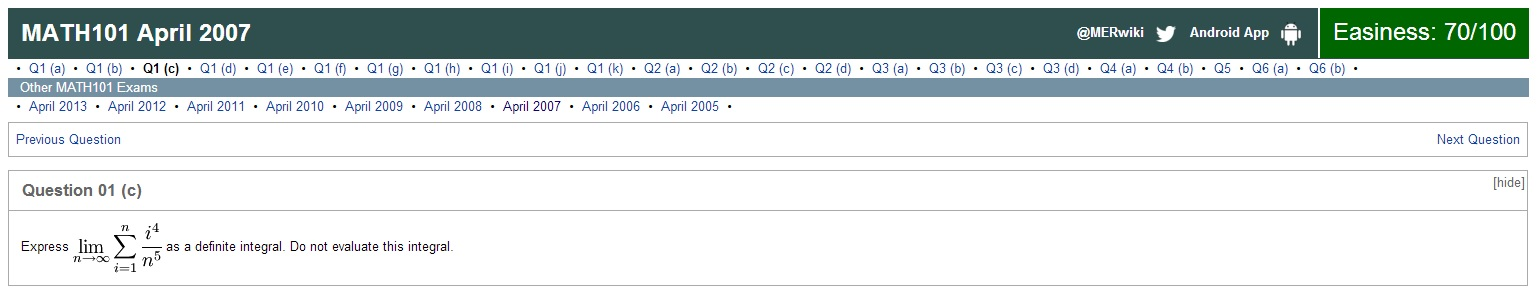
\includegraphics[width=\textwidth]{figs/easiness_rating.jpg}
\caption{The rating for a question is shown in the top right-hand corner of a question. The value is displayed in a colour gradient from green to red with green representing very easy problems and red representing very difficult problems.}\label{fig:Rating_bar}
\end{figure}

\noindent{}The average easiness rating of each question is also displayed in the list of questions on the topic pages (Figure \ref{fig:wiki_tags}). This allows users to personalize and focus their learning even more by choosing questions at an appropriate difficulty level in a particular topic. After completing the questions, students can compare their mastery of the material to the listed score and reassess their study directions based on where their personal rating measures in relation to the group.

\subsubsection{RATING BAR CORRELATION}\label{sec:correlation}
The rating information can be exploited in a way that goes beyond student community engagement. In particular, it can be useful to instructors by correlating student ratings with actual exam scores. For the April 2013 Math 103 exam (Integral Calculus with Integral Calculus with Applications to Life Sciences), anonymized student exam score data was made available. This data can be compared to the MER user score rating for the same exam using student evaluations in the following year (January-April 2014). Figure \ref{fig:score_compare} shows the actual exam score of the 2013 class and the perceived question difficulty of the 2014 class, both scaled to 100.

\begin{figure}[H]
\centering
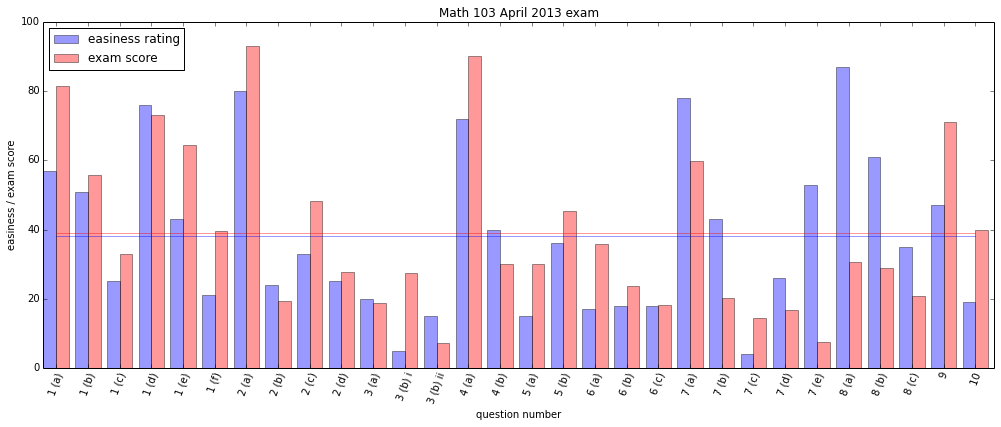
\includegraphics[width=\textwidth]{figs/score_compare.png}
\caption{The actual exam score average for the April 2013 exam is shown in red (the right-most bars) while the corresponding exam rating for the April 2014 class is shown in blue (the left-most bars).}\label{fig:score_compare}
\end{figure}

\noindent{}For each question, the left (blue) bar is the user average easiness rating which could be interpreted as the average prediction that students have about how they would score on this question if it were the exam, and the right (red) bar is the average score that was actually received by students taking that exam in 2013. The horizontal lines are the average score over all questions. These lines are fairly close indicating that overall, students perform slightly better on the final exam than during their exam preparation. In general, it can be seen that the easiness ratings are similar to exam performance. However, Figure \ref{fig:score_compare} highlights some interesting outliers. Question 7(e) has a significantly lower score than perceived difficulty. It could be hypothesized that this is due to the fact that question 7 builds on itself as the student progresses. Therefore, a poor performance on previous parts of the question, as indicated by the negative trend in score as the question progresses, would ultimately hinder the student by the end. However, when using the MER, students can attempt questions independently since all of the previous solutions would be available. This type of rating and score discrepancy could be valuable to instructors in indicating poor test design. It could also be used to help identify false negatives, course topics that are perceived as poorly understood by the students but in actuality are not. Question 8 is also a significant outlier to the data set. This question regards applications of the fundamental theorem of calculus. The first part of the question is perceived as fairly easy by the 2014 student cohort despite the poor performance in 2013. However, the last part of the question, which is much less straightforward, has a stronger correlation between perception and score. It is possible that this data indicates the 2013 student cohort generally underperformed on applications of the fundamental theorem of calculus while these issues were resolved for the 2014 class. Taking that hypothesis as true, the data could indicate that the last part of the question was a difficult problem irrespective of fluctuation in student cohort.
\\\\
\noindent{}In Figure \ref{fig:lin_reg} a linear regression analysis is plotted between the actual 2013 exam scores and the student ratings from 2014. The blue dashed curve represents a perfect linear correlation between the two samples while the red solid curve represents the true curve of linear regression between the data. The slope of the red solid linear regression is less than one and crosses the blue dashed line close to the average scores. Having the slope less than one indicates that students perform worse on questions that they perceive as easy and better on questions that they perceive as hard. This could be a reflection of psychological bias on judging self-performance but more study is warranted or perhaps instructors tend to mark harder questions with greater lenience. The value $p=1.8\times 10^{-4}$ is small so we reject the null hypothesis that there is no correlation between student perception and actual performance. The value $r^2=0.4$ indicates that about 40\% of the exam score data can be explained by student perception. This small correlation study indicates the immense power that the rating system can have on exam and curriculum development. It is of interest to increase the experiment further by incorporating more data sets and looking at other courses.

\begin{figure}[H]
\centering
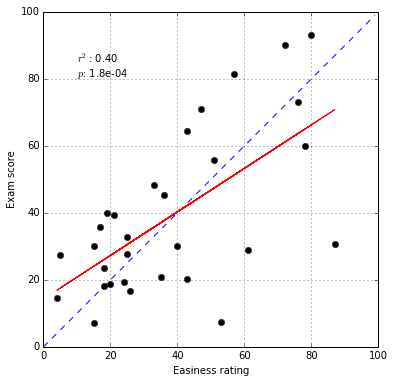
\includegraphics[width=\textwidth]{figs/lin_reg.png}
\caption{Linear regression analysis (solid red line) between the actual exam score average for the April 2013 exam and the exam rating of students in the April 2014 class. The $p$ value is $1.8\times 10^{-4}$ and the $r^2$ value is 0.4. The blue dashed line represents perfect correlation.}\label{fig:lin_reg}
\end{figure}




\subsection{STUDENT CONTRIBUTIONS AND SUSTAINABILITY}\label{sec:Student_Contributions_and_Sustainability}
One of the most challenging aspects of a large volunteer-coordinated open project is that working hours are limited. Furthermore, since the workforce consists primarily of graduate students, there are restrictions due to degree completion timelines. In an effort to alleviate some of these constraints, it would be useful to find a mechanism that transfers the creation process to the same community that uses the service, that is, turn the user into a contributor. One obvious attempt might be to open the wiki for editing by the public, in the way that Wikipedia and other public wikis are. However, in this situation, as university mathematics is a specialized field, there are concerns about the pedagogical standard in the presentation of hints and solutions, not to mention technical challenges like using the typesetting software LaTeX. Thus, when it came to sustainability, other pathways were sought on how undergraduate students can be empowered to contribute meaningfully. Two strategies were recently implemented to increase student contributions and long-term project sustainability, namely the implementation of a solution writing contest and the incorporation of content created through communication grades in a course. Both strategies are described below.
\\\\
\noindent{}During the 2014 April exam period, a solution writing contest for undergraduate students was held. The students could propose solutions to exam problems that were not yet on the wiki and submit them via an online form. These solutions entered the usual peer-review process and eventually became part of the wiki. The aim of this contest was to reduce the workload of content generation and free up time for editing and polishing work to improve its overall quality. Students could submit as many solutions as they wanted and every solution with educational value resulted in a ballot for the authoring student. At the end of the contest there were 22 submitted solutions and three ballots were selected at random to win gift certificates to food services on campus. The winners were advertised on the MER wiki to hopefully generate an even stronger interest in future iterations of the contest. In addition to alleviating the workload on contributors, this contest generated interest from students on continuing their work as some students inquired about a more permanent role in creating solutions.
\\\\
\noindent{}Another approach was implemented by Iain Moyles when he was teaching a third year course on linear algebra. Realising the importance of being able to converse about mathematical concepts with peers, he devoted 10\% of the course grade to a mathematics communication project. To obtain this grade, students had to write solutions to previous exams for the course, in a similar style to exam solutions published on the MER wiki. Thus students were transformed from users to wiki contributors. They were expected to independently work on their solutions at any point through the term. To ensure a high solution quality, a second portion of the grade was to critique the solutions of their peers in a way similar to the peer-review system used in the wiki. The class had 110 students enrolled and this lead to a generation of over 300 solutions. The MER wiki itself uses LaTeX which is a hurdle for users new to typing mathematics, not to mention the additional overhead of creating question pages and managing review flags. To alleviate this barrier, a third-party forum site was chosen to facilitate the logistics of entering their solutions. The forum offers a generous LaTeX toolbar and an organizational scheme that makes it easy to tell when other students have reviewed problems. Course surveys at the end of term showed this idea was well received as students remarked they were essentially getting grades to study and that many would have done the old exam questions anyway in a preparation for their final exam. Many also remarked that having to develop solutions from an instructional perspective led to a deeper understanding of the course material. This idea has great potential; by splitting the workload over a large number of people, the total content was increased by about 25\% in a time period of only two months.
\\\\
\noindent{}This list of features is by no means exhaustive and many new ideas and applications are always being developed. Often, as instructors incorporate the wiki into their teaching, new features emerge organically. For example, Carmen Bruni developed a syllabus for Math 103\footnote{see \url{https://github.com/cbruni/MATH-103-Syllabus-UBC-}}, an integral calculus course for life science students offered at UBC. It was unique in that the document contained learning goals intertwined with sample problems to reinforce the learning objectives and these problems came with a solutions guide. Additionally, at the end of each section, there was a link to the wiki topic pages where students could see the aforementioned videos and question pages on the topics covered in the relevant chapter of the course. This innovative classroom feature was then extended to the wiki with the inclusion of a dynamic syllabus.


\section{USAGE DATA}\label{sec:Usage_Data}
To measure usage of the UBC wiki, user data is collected via Google Analytics. The MER wiki has been analyzed to gain insight into when, how, and how much students use the resource over the duration of their course. In this section the available data is displayed along with a discussion of how it could be used to understand how students approach mathematics problems in general and how they prepare for final exams in particular. Since the MER is being developed at the University of British Columbia, the data is naturally provided for courses offered there. However, it is emphasized that the focus of the presentation is on the types of analytics attainable as well as the general conclusions from data. There is no presumption of general interest in any of the specific data geared to courses at UBC.

\begin{figure}[H]
\centering
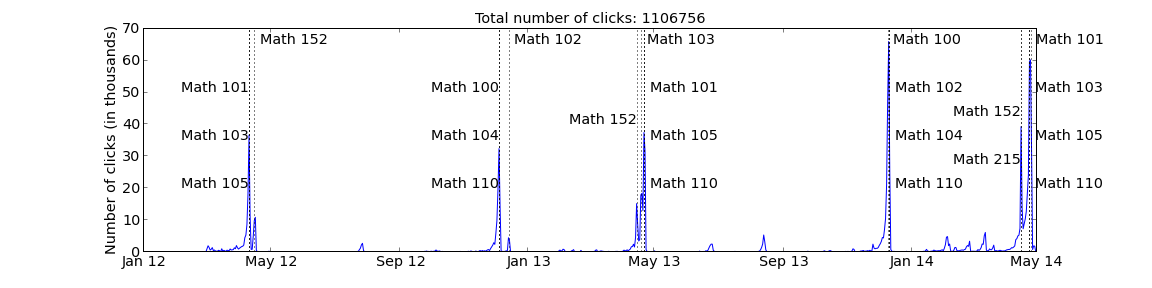
\includegraphics[width=\textwidth]{figs/total_number_of_clicks_time_series.png}
\caption{This shows the total amount of times users clicked something on the MER wiki as a function of time. The exams during the fall and winter terms are also overlay. There is a strong agreement between exam times and wiki usage. Small spikes throughout the year correspond to the summer exam period or midterm examinations.}\label{fig:total_number_of_clicks_time_series}
\end{figure}

\noindent{}Figure \ref{fig:total_number_of_clicks_time_series} shows the total number of times any MER wiki page was accessed (single page request, or click) since its inception on February 20th 2012. Comparing the corresponding terms from 2012, 2013 and 2014, there is a steady increase in the overall wiki use. This is most likely due to a combination of several factors, mainly an increase in the number of available questions, word of mouth as previous users recommend the resource to new students, and improved marketing. Overlying the dates of the final exam, it is evident that the usage is building up to and peaking just before the final exam. Note, however, that the more recent term also show several small peaks around the time of the midterms, a result of the initiative towards transforming the wiki to a general educational resource by adding features such as dynamic syllabi and topic pages.


\begin{figure}[H]
\centering
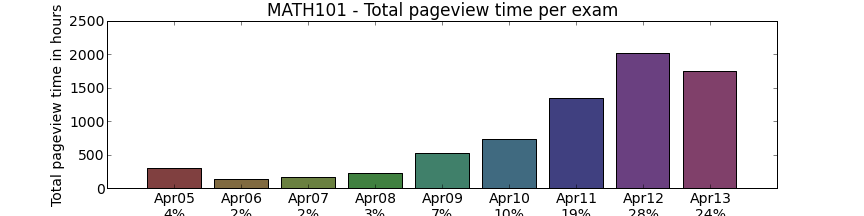
\includegraphics[width=\textwidth]{figs/total_pageview_per_exam_101.png}
\caption{This shows all the exam viewings for a single course Math 101 at the University of British Columbia.}\label{fig:total_pageview_per_exam_101}
\end{figure}

\noindent{}To understand how students use the wiki, a plot of the total time spent per exam, cumulatively on all corresponding question pages is shown in Figure \ref{fig:total_pageview_per_exam_101} for Math 101. Note that the April 2013 exam was not available until early 2014. It shows that students use the most recent exams when preparing for their finals. While historically, the core concepts for each course have remained relatively static, using the most recent exams is likely a reflection of the students’ expectations that the testing style is most relevant with exams chronologically closer to their own. A useful consequence of the data in Figure \ref{fig:total_pageview_per_exam_101} is that any department or institution that wants to implement a platform like the MER can concentrate their efforts on recent exams to generate the strongest student engagement.

\begin{figure}[H]
\centering
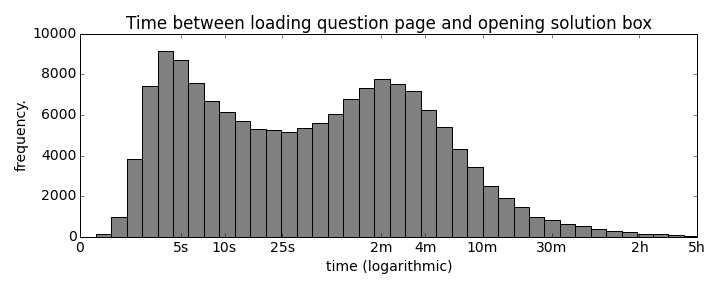
\includegraphics[width=\textwidth]{figs/2013_Term2_delta_t.png}
\caption{This shows the time differential between when a student enters a question page anywhere on the MER wiki and when they click the solution. This data is for the exam period of April 2014 only.}\label{fig:2013_Term2_delta_t}
\end{figure}

\noindent{}When a question page is loaded the solution box is initially closed. In order to see if students solve questions one-by-one on their computer, the delay between page load and opening of the solution box is plotted in Figure \ref{fig:2013_Term2_delta_t}. Noting the logarithmic x-axis, there are two peaks in this time delay, the first around a few seconds, and the second around a few minutes. This data may suggest that a large group of students do not solve the exam questions independently, but rather work through the given solutions or that they work on the questions offline and only afterwards open the solution to check their work. At the same time, it is not uncommon to see students spend several minutes with the problem and hints before checking the solution, which may indicate that a large group of students do work through the problems one-by-one on their computer.

\begin{figure}[H]
\centering
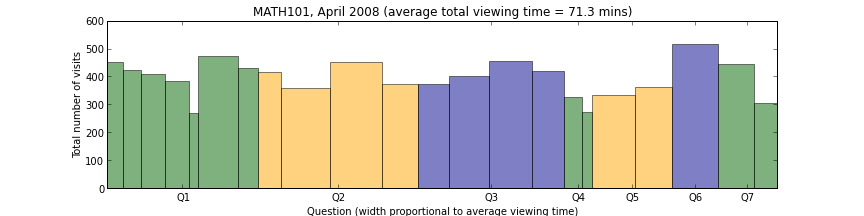
\includegraphics[width=\textwidth]{figs/question_dist_MATH101April_2008.png}
\caption{This is a question breakdown for the April 2008 Math 101 exam at the University of British Columbia. The height of the bars indicate the number of times the question was viewed while the width of the bars indicates the average time spend on that particular question. The colour coding indicates that the question had multiple parts.}\label{fig:question_dist_MATH101April_2008}
\end{figure}

\noindent{}Figure \ref{fig:question_dist_MATH101April_2008} shows the average total viewing time of each question page for the Math 101 April 2008 exam. The motivation for this statistic is the assumption that students keep a page open while they are working on a problem. Therefore, it is reasonable to infer that questions with large times could be difficult to solve or are unclear. In the figure, Question 1 is a short-answer question, where each part is worth the same number of points. Question 1(f)\footnote{see \url{http://wiki.ubc.ca/Science:Math_Exam_Resources/Courses/MATH101/April_2008/Question_1_(f)}} stands out as a short-answer question where students spend most of their time. In fact, it takes students about as long to complete this question as the longer question 6. This may or may not have been intended by the composer of the exam, but having a wiki that tracks usage data allows instructors to automatically gather this kind of information. This could allow future instructors to decide on a reasonable question length and analyze which questions are suitable for the exam time allotted for short-answer questions. The other questions that stand out in this graph for receiving a very low average time are Q1(e) (probability) and Question 4 (higher order differential equations), which are both on topics that have been removed from the course curriculum as of 2009. It is worth emphasizing again that the specific data in Figure \ref{fig:question_dist_MATH101April_2008} is likely not of any interest to mathematics educators outside of the University of British Columbia. However, the ability to analyze a subset of questions in terms of viewing time and time spent on questions can have significant impacts on exam development and efficient utilization of educational resources (teaching assistants, workshops, etc.).

\section{IMPACT ON STUDENT LEARNING}
A Teaching and Learning Enhancement Fund (TLEF) was awarded to the authors to design and perform learning impact studies on the MER wiki. While the majority of analytic results and implications of this study are still under development, it is worth discussing some preliminary results. Specifically, part of the study included surveys about MER usage and its effectiveness as a learning tool. Three open ended questions asked on the survey were

\begin{enumerate}
\item What features do you like best?
\item How can we improve the MER wiki?
\item What impact do you perceive the MER wiki has on your mathematics learning?
\end{enumerate}

\noindent{}and they were answered by 91 participants. The overall consensus of students was that the MER was well organized and easy to use, and that the solutions provided a strong amount of detail promoting their understanding of mathematics. Two specific excerpts of students comments on solutions were

\begin{quote}
\textit{[I like] The fact that each question has detailed solutions. This is extremely helpful for clarifying concepts and understanding how to approach questions.}

\textit{if I can't figure out a solution after exhausting every possibility, it is extremely helpful to me to understand where EXACTLY I went wrong in a specific problem.}
\end{quote}

\noindent{}Students were similarly pleased with the hints. One particularly useful comment was

\begin{quote}
\textit{Hints are very useful compared to doing textbook questions where you can only compare with solutions.}
\end{quote}

\noindent{}This once again highlights the advantage over the MER as compared to a standard print textbook which is a static medium. Contributors to the MER can add and edit hints to support student development at any point. In terms of suggested improvements, some interesting responses were as follows:

\begin{quote}
\textit{I would like to see more practice midterm exams in addition to the final exams that are already available.}

\textit{Final Exam Solutions because the math club solution book that they sell always has multiple errors.}

\textit{I would like to see a comment system so that students can share what parts of the problem they found difficult.}
\end{quote}

\noindent{}The student’s comment about solutions referred to the final exam answer as opposed to the whole solution. Many students were interested in having access to this because they did not want to read the whole solution to see if they had completed the problem correctly. Furthemore, many students who did solve the problem incorrectly wanted to make future attempts on their own. Having to read through the solution to check their answer had the potential to negatively impact their study habits by being prematurely exposed to the correct way to solve the problem. Since this set of comments, an algorithm has been developed to extract the final answer from a problem and include an option to display the answer without the solution.
\\\\
\noindent{}The students’ request for midterm questions has a fairly strong voice as well. Since midterm questions are often styled the same as exam questions, this request may well simply be asking for an increase in content. While there are over 1500 worked solutions, once these are broken into categories it can leave limited options for students to study specific topics. It is a future MER direction to address these issues. The last comment regarding the desire for a discussion system with students may reflect a poor advertisement of the discussion feature that already exists or a desire to have something that is solely available to students and not moderated by contributors. Either way, it has become a focus of the MER team to evaluate the implementation of the discussion system.
\\\\
\noindent{}In regards to impact on student learning, it was a generally observed trend that students were certain the MER had a positive impact on their education but they could not properly describe in what way. It is worth noting that a voluntary survey like this is susceptible to self-selection bias. However, this merely demonstrates that there are groups of students who view the MER as a valuable resource for their learning, indeed some claimed that it was the best learning resource. There is no assertion that the MER is or would be the best resource for all students but rather that it offers another medium for positive learning impact on students. The following were a variety of responses offered by survey participants in regards to impact on student learning:

\begin{quote}
\textit{I feel that the MER wiki has had a significant positive impact on my math exam performance as it provides detailed solutions to problems I might not have otherwise been able to solve.}

\textit{I feel that the MER wiki helps build my confidence and speed when doing questions. This really helps when you are pressed for time during a midterm or final.}

\textit{It's useful for my homework.}

\textit{The alphabetical list of topics is also very beneficial because by clicking on the links, you have a rough idea of which "specific" topic(s) you might be having trouble with. On the flip side, you also have a rough idea of which "specific" topic(s) you have mastered. It definitely improves it. It’s very helpful.}

\textit{It [the MER wiki] has been a positive impact for me. The videos on specific topics helped me understand concepts I may not have fully grasped from listening to my instructor. It is helpful to learn from different sources. It helps me a lot!}

\textit{It's good to have other resources than the instructor no matter what time it is.}
\end{quote}

\noindent{}The summary of student learning impact, as observed from the students themselves anecdotally, indicates that there is a perceived positive impact from the MER. Many of the features that the authors speculated to being useful were corroborated by these statements and other similar comments. Further analysis of the full survey data is warranted and indeed is in preparation. Student testimonials are also currently being analyzed, which will offer a deeper insight into some of the answers provided with which the above quotes were sampled.

\noindent While it is beyond the scope of this paper and indeed the scope of the current student impact study, there has been some ongoing interest in soliciting similar feedback from instructors.  Some important questions that would be of interest here are the MER’s impact on student learning as perceived by instructors and, from a pedagogical perspective, the MER’s potential for exam and curriculum development.


\section{CONCLUSIONS}\label{sec:Conclusions}
Throughout its history, the MER wiki has been evolving from a static exam review resource to a dynamic content collection with significant potential for future improvements and growth. An online resource has been created where students can study mathematics via worked examples, watch related videos and impact the available content directly through their feedback. Students come to the wiki with a basic theoretical knowledge/background and are then able to work through problems, guided by hints and thorough solutions, an interactive syllabus for their course, videos, and the easiness ratings of their fellow students. In addition, they can submit questions and suggestions about the content and rate problems themselves.
\\\\
\noindent{}The continual growth and improvement of the MER means that future directions are always being considered. Some future directions for the project include a deeper analysis of the impact study, personalization through computer-generated, individualized learning plans for students, more data analysis for exam and curriculum improvement, and a drive for stronger student engagement through community generated content.
\\\\
\noindent{}For all its potential, the future success and development of the MER wiki requires a paradigm shift, as it develops a new mathematics education culture of accessibility in alternative mediums. The MER wiki represents a significant deviation from traditional resources available to students outside of the classroom and some instructors, administrators and decision-makers may be reluctant to embrace these changes or participate in the new culture. In addition, despite research that shows its effectiveness as a learning tool, some may have reservations about posting worked problems, the primary content offering. Through previous discussions and observations of student comments, it suggests that the wiki structure with background material, hints, and solutions does facilitate student learning and offers a lot of potential for improving the undergraduate mathematics education experience.
\\\\
\noindent{}In \cite{PM}, a study was conducted that measured test performance between groups of students with a variable training of worked examples.  Their conclusions suggest that studying from worked examples reduced the cognitive load on students when compared to conventional problem solving strategies, that is,  not having the solutions provided.  The participants were chosen from a specific senior level programming course at a Netherlands secondary school and were composed of 58 men and 2 women.  The top test scorer was rewarded with a cash prize.  Critics of research into the effectiveness of worked examples using a study such as as conducted in \cite{PM} could argue about a variety of biases introduced by the nature of this experimental design.  Likely, by selecting a senior level programming course, there was a bias towards stronger students.  In this particular study women were underrepresented, and offering a financial incentive could have skewed the student engagement from a natural study environment.  One of the benefits of the MER is that similar studies such as \cite{PM} and the other references of this manuscript can be conducted in a more passive way.  Since analytics are constantly measuring quantitative variables such as time spent on a page or links that are clicked, data can be collected on students at any time while they are studying in their natural environment.  Furthermore, at UBC and many other institutions, first year calculus classes are a general requirement for most programs and therefore, we are able to collect data from a variety of learners with different mathematical skills and interests.  By conducting surveys and interviews we are able to capture more specific details about the data we’re collecting, including demographics, so that we can correct for any bias that may be introduced.   Overall, combining data and conclusions from the MER with previous studies of worked examples strengthens the arguments of positive benefits of worked examples and helps alleviate concerns that can arise in transitional simulated studies. The marriage of content, technological innovation, and accessibility on the MER wiki allows for a modern interpretation and analysis of classroom trial studies of worked examples and represents one face of the future of education. 
\\\\
\noindent{}Having an education resource which collects data at the scale that the MER provides a mechanism to bring data into educational research questions. However, concurrently, access to this data generates research questions on its own. Two such questions that the data presented in this paper could generate are as follows. Firstly, while the students’ ability to rate questions could provide an interesting resource to instructors, they could also impact student use of the resource and their study habits. Specifically, it is worth investigating if students avoid certain questions that are rated too difficult. Conversely, students may be spending too long solving problems with an easy rating to artificially inflate their mathematical confidence. If they struggle on a problem that is rated very easy then this could negatively impact their confidence and frustrate their study habits. A second question that arises is from the dataset provided in Figure \ref{fig:2013_Term2_delta_t} which has bimodal peaks from users who open the solution right away and users who open it after some amount of time has passed. While difficult to analyze, it is a valid question to ask how students in these two bimodal categories score on the actual exam and in the course. This may have general implications to the role of worked examples.
\\\\
\noindent{}This resource is constantly changing and evolving. Even at the time of reading, the wiki has likely changed, expanded and improved in usability and sustainability. It is this dynamic feature of the wiki that makes it a truly amazing project to be a part of and to watch develop into a widely used resource for undergraduate students. This group of authors cannot wait to see how the future of this resource can be used to shape new generations of mathematicians. They also hope that other institutions will implement a similar structure or find ways to interface with the MER.

\section{ACKNOWLEDGEMENTS}\label{sec:Acknowledgements}
On title page.


\begin{thebibliography}{1}

\bibitem{CS2}
Graham~A. Cooper.
\newblock Effects of schema acquisition and rule automation on mathematical
problem-solving transfer.
\newblock {\em Journal of educational psychology}, 79:pp. 347 -- 362, 1987.

\bibitem{PM}
Fred~GWC Paas and Jeroen~JG Van~Merri{\"e}nboer.
\newblock Variability of worked examples and transfer of geometrical
problem-solving skills: A cognitive-load approach.
\newblock {\em Journal of educational psychology}, 86(1):122, 1994.

\bibitem{CS1}
John Sweller and Graham~A. Cooper.
\newblock The use of worked examples as a substitute for problem solving in
learning algebra.
\newblock {\em Cognition and Instruction}, 2(1):pp. 59--89, 1985.

\end{thebibliography}

%\bibliographystyle{unsrt}
%\bibliography{bib}

\section*{APPENDICES}

\appendix

\section{WIKI IMPLEMENTATION}\label{sec:Appendix}

This appendix will briefly discuss the implementation of the MER wiki, with an emphasis on how particular aspects of the MediaWiki platform were utilized to meet the design needs.
\\\\
\noindent{}One of the foundational design choices of the wiki was putting each question along with its associated hints and solutions on an individual Question page. Question pages are grouped as subpages of their originating exam, and exams are grouped as subpages of their respective courses. All course pages are linked to from the front page of the resource, which also displays a summary of the amount of available content for each course.
\\\\
\noindent{}MediaWiki’s template and transclusion functionality is the fundamental building block used to implement the design scheme described above. Transclusion is a MediaWiki feature in which the content of a wiki page can be embedded in another page. Templates are a special type of wiki pages meant for transclusion in other wiki pages, creating identically formatted pages whose source code is in one location. Templates were used to frame most pages on the MER wiki, most notably the individual question pages. Implementing the question page as a template means that if a change to the layout of the question pages is desired, the only thing required is to edit the template and changes will be reflected on all the pages created with that template.
\\\\
\noindent{}The other primary MediaWiki feature used to construct the MER wiki is categories. Categories are essentially tags that can be added to wiki pages; clicking on the tag will then list all pages with that tag. Category tagging was used in multiple ways on the wiki. Categories facilitate the peer review process: each stage in the peer review process has a corresponding category, and question pages are tagged with the appropriate categories to indicate their progress in the peer review process. The topic tagging system of the wiki was also implemented using the categories feature. Finally, categories are used as an organizational tool to keep track of our pages, templates and contributors.
\\\\
\noindent{}Another advantage of the MediaWiki platform is the availability of free extensions that allow for the addition of extra features. These include features as fundamental as the ability to render LaTeX in wiki pages to the advanced level of having a ratings bar for students to rate questions. The DynamicPageList extension has also been foundational in how the MER wiki is organized and how content is presented. Other useful extensions used include: PageInCat, ParserFunctions, RightFunctions, Variables, Widgets and Category Tree.
\\\\
\noindent{}In addition to focusing on student usability, this resource was also built with the requirements of efficient editing in mind, including an online peer review system and space for contributors to communicate and organize tasks. For the latter, a separate set of wiki pages for administrator and contributor use was created. These pages help us to keep track of which courses need to be updated as well as keep track of current open projects for the wiki. These pages include links to a contributor’s and developer’s manual which features a multiple-series how-to-contribute videos on youtube. In addition, while most of the content related tasks (adding and editing solutions, creating new exams) are managed through these dedicated wiki pages for contributors, much of our development work has been organized through other online tools, notably Google Drive (for web forms and general documents) and a project management app named Hojoki that helps to organize the tasks. For more information on the design or implementation, please see the complete developer’s manual at \url{http://wiki.ubc.ca/Science:MER/Manual}.
\end{document}